%%%%%%%%%%%%%%%%%%%%%%%%%%%%%%%%%%%%%%%%%%%%%%%%%%%%%%%%%%%%%%%%%%%%%%
% LaTeX Example: Project Report
%
% Source: http://www.howtotex.com
%
% Feel free to distribute this example, but please keep the referral
% to howtotex.com
% Date: March 2011 
% 
%%%%%%%%%%%%%%%%%%%%%%%%%%%%%%%%%%%%%%%%%%%%%%%%%%%%%%%%%%%%%%%%%%%%%%
% How to use writeLaTeX: 
%
% You edit the source code here on the left, and the preview on the
% right shows you the result within a few seconds.
%
% Bookmark this page and share the URL with your co-authors. They can
% edit at the same time!
%
% You can upload figures, bibliographies, custom classes and
% styles using the files menu.
%
% If you're new to LaTeX, the wikibook is a great place to start:
% http://en.wikibooks.org/wiki/LaTeX
%
%%%%%%%%%%%%%%%%%%%%%%%%%%%%%%%%%%%%%%%%%%%%%%%%%%%%%%%%%%%%%%%%%%%%%%
% Edit the title below to update the display in My Documents
%\title{Project Report}
%
%%% Preamble
\documentclass[paper=letter, fontsize=10pt]{scrartcl}
\usepackage[body={7in,7.5in},top=1in, bottom=1in]{geometry}
\usepackage[T1]{fontenc}
\usepackage{fourier}

\usepackage[english]{babel}															% English language/hyphenation
\usepackage[protrusion=true,expansion=true]{microtype}	
\usepackage{amsmath,amsfonts,amsthm} % Math packages
\usepackage[pdftex]{graphicx}	
\usepackage{url}
\usepackage{enumerate}
\usepackage{lastpage}
\usepackage{float}
\usepackage{hyperref}


%%% Custom sectioning
\usepackage{sectsty}
\allsectionsfont{\normalfont\scshape}


%%% Custom headers/footers (fancyhdr package)
\usepackage{fancyhdr}
\pagestyle{fancy}
\fancyhead[L]{}
\fancyhead[c]{Design Revision 0 Revision 0}
\fancyhead[R]{\today}											
\fancyfoot[L]{}											 
\fancyfoot[C]{}											
\fancyfoot[R]{\thepage\ of \pageref{LastPage}}		% Pagenumbering
\renewcommand{\headrulewidth}{0.4pt}				% Remove header underlines
\renewcommand{\footrulewidth}{0.4pt}				% Remove footer underlines
\setlength{\headheight}{13.6pt}


%%% Equation and float numbering
\numberwithin{equation}{section}		% Equationnumbering: section.eq#
\numberwithin{figure}{section}			% Figurenumbering: section.fig#
\numberwithin{table}{section}				% Tablenumbering: section.tab#


%%% Maketitle metadata
\newcommand{\horrule}[1]{\rule{\linewidth}{#1}} 	% Horizontal rule
\newcommand{\ts}{\textsuperscript}

%%% Begin document
\begin{document}

\begin{titlepage}

\newcommand{\HRule}{\rule{\linewidth}{0.5mm}} % Defines a new command for the horizontal lines, change thickness here
\newcommand{\authors}{\shortstack{Vitaliy Kondratiev,\\Nathan Johrendt,\\Tyler Lyn,\\Mark Gammie}}

\begin{center}
 
%----------------------------------------------------------------------------------------
%	HEADING SECTIONS
%----------------------------------------------------------------------------------------

\textsc{\LARGE McMaster University}\\[1.5cm] % Name of your university/college
\textsc{\Large CAS 4ZP6}\\[0.5cm]
\textsc{\Large Team 9} \\[0.5cm]
\textsc{\Large Capstone Project 2013/2014}\\[0.5cm] % Major heading such as course name
\textsc{\large Porter Simulation}\\[0.5cm] % Minor heading such as course title

%----------------------------------------------------------------------------------------
%	TITLE SECTION
%----------------------------------------------------------------------------------------

\HRule \\[0.4cm]
{ \huge \bfseries Design Revision 0}\\[0.4cm] % Title of your document
\HRule \\[1.5cm]
 
%----------------------------------------------------------------------------------------
%	AUTHOR SECTION
%----------------------------------------------------------------------------------------

\begin{minipage}{0.4\textwidth}
\begin{flushleft} \large
\emph{Authors:}\\
Vitaliy Kondratiev - 0945220\\
Nathan Johrendt - 0950519\\
Tyler Lyn - 0948978\\
Mark Gammie - 0964156\\
\end{flushleft}
\end{minipage}
~
\begin{minipage}{0.4\textwidth}
\begin{flushright} \large
\emph{Supervisor:} \\
Dr. Douglas Down % Supervisor's Name
\end{flushright}
\end{minipage}\\[4cm]

% If you don't want a supervisor, uncomment the two lines below and remove the section above
%\Large \emph{Author:}\\
%John \textsc{Smith}\\[3cm] % Your name

%----------------------------------------------------------------------------------------
%	DATE SECTION
%----------------------------------------------------------------------------------------

{\large \today}\\[3cm] % Date, change the \today to a set date if you want to be precise

%----------------------------------------------------------------------------------------
%	LOGO SECTION
%----------------------------------------------------------------------------------------

%\includegraphics{Logo}\\[1cm] % Include a department/university logo - this will require the graphicx package
 
%----------------------------------------------------------------------------------------
%Template taken from: http://www.softwaretestinghelp.com/test-plan-sample-softwaretesting-and-quality-assurance-templates/

\vfill % Fill the rest of the page with whitespace
\end{center}
\end{titlepage}

\setcounter{tocdepth}{2}

\tableofcontents

\newpage

\section{Revision History}
\begin{center}
    \begin{tabular}{| c | l | l | p{5cm} |}
    \hline
    Revision \# & Author & Date & Comment \\ \hline
  	1 & \shortstack{\\Vitaliy Kondratiev,\\Nathan Johrendt,\\Tyler Lyn,\\Mark Gammie} & January 11, 2014 & Revision 0 Added to repository \\ \hline
  	2 & \shortstack{\\Vitaliy Kondratiev,\\Mark Gammie} & January 12, 2014 & Added diagrams to Latex \\ \hline
  	3 & \shortstack{\\Tyler Lyn} & January 12, 2014 & Added dispatch module \\ \hline
  	4 & \shortstack{\\Vitaliy Kondratiev,\\Nathan Johrendt} & January 13, 2014 & Added GUI Component to document \\ \hline
  	5 & \shortstack{\\Mark Gammie} & January 13, 2014 & Updated Dependency Diagram to contain algorithms and data structures. Updated dependency diagram with a legend, logging comment and fixed the porter dispatcher dependency \\ \hline
  	6 & \shortstack{\\Tyler Lyn,\\Mark Gammie} & January 13, 2014 & Several Modules Updated \\ \hline
	7 & \shortstack{\\Nathan Johrendt} & January 13, 2014 & Added Appendix \\ \hline
	8 & \shortstack{\\Mark Gammie} & January 14, 2014 & Completed Design Overview\\ \hline
        
    \end{tabular}
\end{center}

\section{Executive Summary}
\subsection{Introduction}
This document outlines the design decisions, style and methodology for the project of Porter Simulation to be completed for Hamilton Health Sciences.  A modular design methodology has been chosen as our design principle.  This document is based on IEEE Draft Standard for Software Design Descriptions (IEEE P1016/D5.0).
\subsection{Purpose}
The purpose of this document is to outline the design of each component and how they interface between each other. This document will aid the developers in the development process as well as any future maintenance required.
\subsection{Design Overview}
Our solution is a discrete event simulation that is implemented using the Python library SimPy. The simulation has three main sections named Import, Export and Core. 

The UI section contains the modules for providing the user interface. The UI is responsible for taking input from the user as well as preventing them from entering erroneous data/ ensuring integrity of the data before releasing it to the simulation core..

The Export section contains a module for reporting statistics that are generated by the simulation. The module will be used after the simulation has completed to write the generated data to a csv file that will be interpreted later by some Visual Basic scripts. These scripts will be used to generate predetermined graphs for the user to view.

The Core section is where the simulation actually occurs. The module Simulation Core contains the command line interface for the simulation and is responsible for initializing the Simulation State, Job List Builder and Dispatcher modules. The Job List Builder module will create a list of jobs using the data contained in the file filled with historical data. This list of jobs will be submitted to the Simulation State to be stored. Once the simulation is started, the Dispatcher module is responsible for receiving the jobs as they become available and assigning them intelligently to any eligible porters. The porters that operate on the tasks follow a finite state machine that creates timeouts based on the time it would take for each state that the porter is transitioning into. There may be cases when all the porters are busy and the amount of assigned jobs piles up, or the porters are stuck waiting on jobs to become available. Once the simulation terminates, the export of the statistical data is finalized.
\section{Implementation Material}
\subsection{Language of Implementation}
Visual Basic in Excel will be used to interface GUI to Simulation Core module. Python Version 2.7.5 will be used for Simulation Core module and all other modules.
\subsection{Supporting Technology and Frameworks}
Simulation will be built on the SimPy 3.0.2 library \newline \ \underline{\url{https://simpy.readthedocs.org/en/latest/}}. GUI will be built in Excel 2010. 

\section{Process Diagram}
\begin{figure}[H]
	\begin{center}
		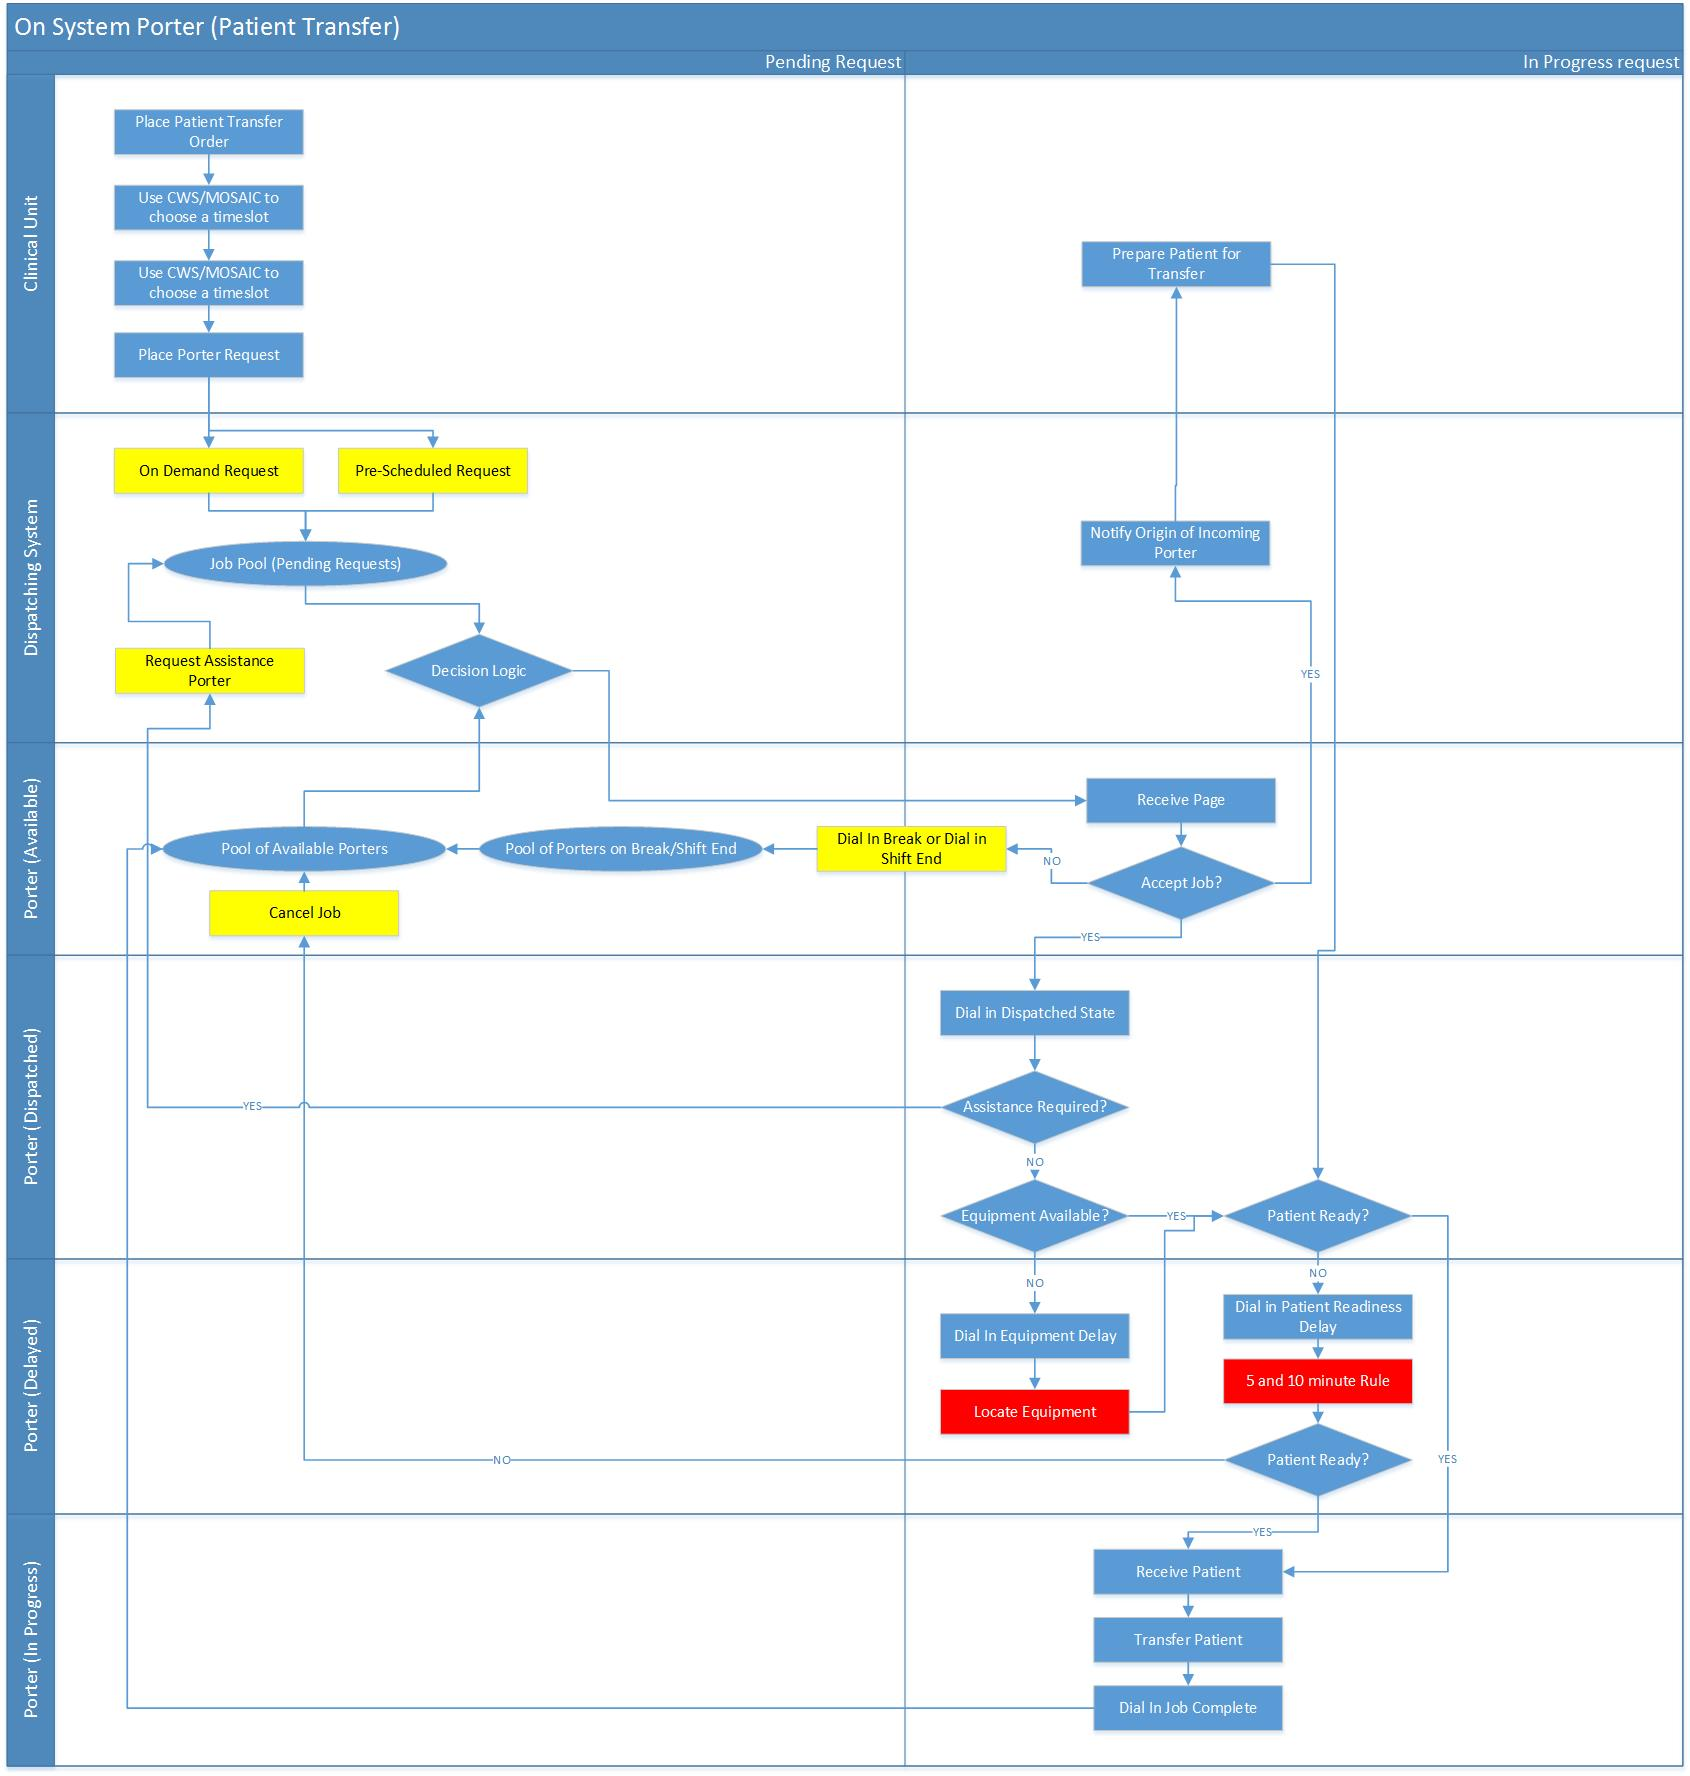
\includegraphics[width=1\textwidth, height=0.8\textheight, keepaspectratio]{../Process_Diagrams/Process_Diagram.jpg}
		\caption{Process Diagram}
	\end{center}
\end{figure}

\section{Dependency Diagram}
\begin{figure}[H]
	\begin{center}
		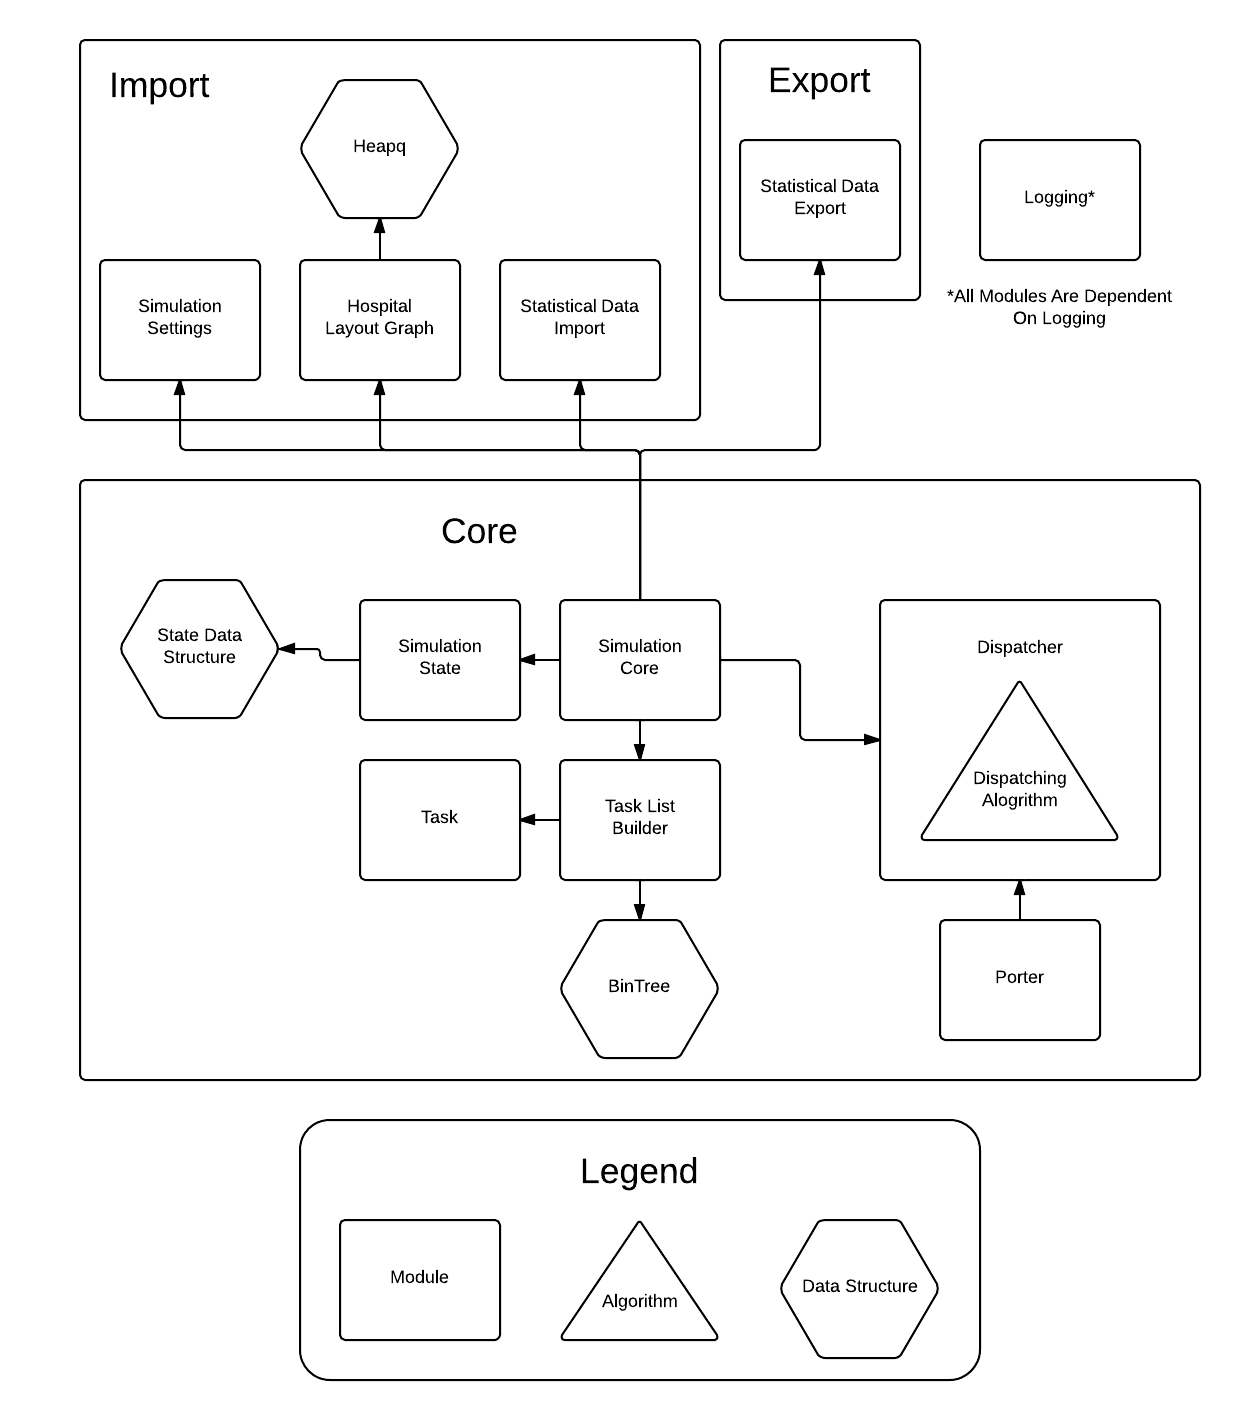
\includegraphics[width=1\textwidth, height=0.8\textheight, keepaspectratio]{../Process_Diagrams/Dependency_Diagram.png}
		\caption{Dependency Diagram}
	\end{center}
\end{figure}

\section{Decomposition Description}
\subsection{Core - Simulation Core}
\begin{enumerate}[]
	\item \textbf{Type:} Module
	\item \textbf{Purpose:} This module calls the required functions to create the Job List, initialize the simulation state and initialize the simulation processes.
	\item \textbf{Function:} This module takes in configuration data from the GUI module and uses it to initiate the required modules Job List Builder, Porter Manager and Dispatcher, and passes their resulting data into the Simulation State.
	\item \textbf{Interface:}\\ 
	The interface to this module is a dictionary containing the information for the configuration of the simulation.
	
	\item \textbf{Process Steps:} This module is passed the configuration data from GUI module. With the configuration data it constructs the Job List, Porter Manager, Dispatcher which will be stored in the Simulation State. Once that has been done, the module will run the simulation for the configured amount of time. At this point, the simulation has completed and the module finishes by running the Statistical Data Export module.
	\item \textbf{Data:} None
	\item \textbf{Error Handling:} Catch all on the simulation loop to report pertinent errors and to prevent unexpected termination. 
	\item \textbf{Requirement Reference:} 11.1.3
\end{enumerate}
\subsection{Core - Simulation State}
\begin{enumerate}[]
	\item \textbf{Type:} Module
	\item \textbf{Purpose:} This module's purpose is to be an interface between the simulation and its simulation state data structure.
	\item \textbf{Function:} This module will contain several objects that will be used by the many modules that are in the simulation.
	\item \textbf{Interface:}\newline
	env:
		\begin{itemize}
			\item A reference to the simpy env object.
		\end{itemize}
	porterManager:
		\begin{itemize}
			\item A reference to the porterManger object.
		\end{itemize}
	dispatcher:
		\begin{itemize}
			\item A reference to the dispatcher object.
		\end{itemize}
	jobList:
		\begin{itemize}
			\item A reference to the jobList object.
		\end{itemize}
	maxDelayReason:
		\begin{itemize}
			\item A dictionary used to look up the max delay for each delay reason.
		\end{itemize}	
	\item \textbf{Process Steps:} This module handles the simulation state data structure and allows the rest of the modules to interact with it.  If modules need information about the simulation as a whole, they will communicate with the Simulation State module in order to satisfy their needs. 
	\item \textbf{Data:} Simulation state data structure
	\item \textbf{Error Handling:} Catch any null values in the simulation state data structure
	\item \textbf{Requirement Reference:} None
\end{enumerate}
\subsection{Core - Job}
\begin{enumerate}[]
	\item \textbf{Type:} Module
	\item \textbf{Purpose:} Provide information about a job to the porter.
	\item \textbf{Function:} The task is declared with an origin, destination, priority, appointment, delay information and state change time values.  This information is necessary to allowing a porter to complete a job.
	\item \textbf{Interface:} \newline
		autoUpdateProcess(simState, au):
			\begin{itemize}
				\item A process that increases the job's priority as it waits to be assigned to a porter based off of the au input.
			\end{itemize}
	\item \textbf{Process Steps:}  Jobs will be initialized within the Job List Builder.   An initialized job will be able to provide the Dispatcher all the required information to assign jobs.  Once a job is given to a porter, the porter will then be able to start and complete a transport job.
	\item \textbf{Data:} Transport Job Information
	\item \textbf{Error Handling:} Catch any null values returned by the task's properties
	\item \textbf{Requirement Reference:} None
\end{enumerate}
\subsection{Core - Job List Builder}
\begin{enumerate}[]
	\item \textbf{Type:} Module
	\item \textbf{Purpose:} Produces the list of jobs for the Simulation Core and Dispatcher modules to process
	\item \textbf{Function:} This module parses the file that contains historical job data and creates list of jobs that are ordered based of their creation time.
	\item \textbf{Interface:} \newline
		runImport(fileName):
		\begin{itemize}
			\item Imports the data from historical job data file and constructs and returns the jobList along with the dispatchTable.
		\end{itemize}
		addDispatchTime(origin, dispatchTime)
		\begin{itemize}
			\item Adds a dispatch time to the dispatchTable
		\end{itemize}
	\item \textbf{Process Steps:} The Job List Builder will first receive the historical data file's file name from the Simulation Core.  This file name will allow the Job List Builder to create jobs based off of historical data.  Secondly, the Job List Builder will generate jobs and insert them into the jobList data structure.  The jobList is responsible for the storage, ordering and releasing of jobs into the dispatcher.
	\item \textbf{Data:} jobList
	\item \textbf{Error Handling:} Catch any null tasks
	\item \textbf{Requirement Reference:} 11.1.1
\end{enumerate}
\subsection{Core - Porter}
\begin{enumerate}[]
	\item \textbf{Type:} Module
	\item \textbf{Purpose:}  To complete jobs provided by the dispatcher
	\item \textbf{Function:} Completes the transport jobs assigned by the dispatcher.  Unless a job is cancelled the porter will traverse through four states ('pending', 'dispatched', 'inprogress', 'complete')
	\item \textbf{Interface:} \newline
	work(simState):
		\begin{itemize}
			\item Input the Simulation State
			\item Finite state machine that causes the Porter to ultimately be locked to the job for the duration of its execution. Will also cancel a job and reschedule it if the porter is waiting too long on the patient. The function will also update state values of the job for storage of the generated statistics.
		\end{itemize}
	\item \textbf{Process Steps:} The module is responsible for representing Porters in the simulation and their ability to perform jobs and perform those jobs according to . This is where the majority of statistically valuable information is generated.
	\item \textbf{Data:} Stores internal data relating to its' current state.
	\item \textbf{Error Handling:} None
	\item \textbf{Requirement Reference:} None
\end{enumerate}
\subsection{Core - Dispatcher}
\begin{enumerate}[]
	\item \textbf{Type:} Module
	\item \textbf{Purpose:} To organize pending jobs based on a weighted-value and assign them to porters 
	\item \textbf{Function:} This module orders pending jobs based off of a Dispatch Value which is computed using several parameters (Weighted Job Priority and Appointment Factor).  The pending job with the greatest Dispatch Value will be assigned to the closest available porter.  Once the job is assigned to the porter the job will be considered a dispatched job.
	\item \textbf{Interface:} \newline
	 assignJob(Task):
	 	\begin{itemize}
	 		\item Assigns the job with the greatest Dispatch Value to the closest available porter.
	 	\end{itemize}
	 getWeightedJobPriority(TaskOrigin, TaskDestination):
	 	\begin{itemize}
	 		\item Input the origin and destination of a pending job
	 		\item Output a value based on the priority of the pending job
	 	\end{itemize}
	 getAppointmentFactor(Task):
	 	\begin{itemize}
	 		\item Input a pending job
	 		\item Update the value for a job depending on if it was pre-scheduled or on-demand.
	 	\end{itemize}
	 getDispatchValue(Task):
	 	\begin{itemize}
	 		\item Input a pending job
	 		\item Compute the DispatchValue for a job: (WeightedJobPriority * AppointmentFactor) 
	 	\end{itemize}
	\item \textbf{Process Steps:}
	All pending jobs are assessed and given a dispatch value (DV) based on the weighting and values of specified dispatch parameters.
	
	These weights and values are determined using either the location of an available porter or the priority of a pending job.
	
	All of the pending jobs are then ordered from greatest dispatch value to the least.  When there is an available porter the pending job with the greatest dispatch value is given to the closest porter.
	\item \textbf{Data:}
		\begin{itemize}
			\item Pending jobs
		\end{itemize}
	\item \textbf{Error Handling:} None
	\item \textbf{Requirement Reference:} None
\end{enumerate}
\subsection{Core - Porter Manager}
\begin{enumerate}[]
	\item \textbf{Function:} This module populates a series of tasks following either a distribution or statistical data.
	\item \textbf{Interface:} \newline
		importPorterSched(self, porterSchedule)
		\begin{itemize}
			\item Input the porter schedule and initialize all of the porters.
		\end{itemize}
		getPendingPorters(self, creationTime):
		\begin{itemize}
			\item Input the creationTime of a job.  Create a list of porters that  are available depending on the creationTime.  
		\end{itemize}
		
	\item \textbf{Process Steps:} The porterManager handles the creation of porters and the availability of porters at a certain time.  Based on the current time in the simulation the proterManager will provide the simulation with the porters who can accept jobs.
	
	\item \textbf{Data:} Porter Schedule
	\item \textbf{Error Handling:} None
	\item \textbf{Requirement Reference:} None
\end{enumerate}

\subsection{Export - Statistical Data Export}
\begin{enumerate}[]
	\item \textbf{Type:} Module
	\item \textbf{Purpose:} Format and output the raw data from the simulation.
	\item \textbf{Function:} This module will gather all of the raw data from the simulation and format it  so that it can be exported into a readable excel file.
	\item \textbf{Interface:}
	publishData(simulationData)
	\begin{itemize}
		\item This function will format the simulation's raw data, create an excel file and populate the file with the formatted data
	\end{itemize}
	\item \textbf{Process Steps:} All data that is to be exported must be added to this module.  Once the simulation's raw data is gathered the module will publish the data.  The publishing will generate an excel file and outline the results from the simulation.
	\item \textbf{Data:} simulationData
	\item \textbf{Error Handling:}  Produce warning message if data is missing during the publishing.
	\item \textbf{Requirement Reference:} 11.1.4
\end{enumerate}

\subsection{Export - Statistical Data Analysis}
\begin{enumerate}[]
	\item \textbf{Type:} Module
	\item \textbf{Purpose:} Outputs an excel dashboard file containing all the statistical analysis
	\item \textbf{Function:} This module will take the excel output and use it construct excel charts and graphs  
	\item \textbf{Interface:}
	runMacros(outputFile)
	\item \textbf{Process Steps:} Record the output data into itself allowing for inside functions to manage the calculations. Create a copy of itself at the user specified location
	\item \textbf{Data:} outputData
	\item \textbf{Error Handling:} Produce warning message if errors occurs during process
	\item \textbf{Requirement Reference:} 11.1.5
\end{enumerate}

\subsection{UI - Basic Settings - General}
\begin{enumerate}[]
	\item \textbf{Type:} User Interface
	\item \textbf{Purpose:} Allows the user to change the basic-general settings of the simulation
	\item \textbf{Function:} Interface will allow entry of basic variables while preventing erroneous entry
	\item \textbf{Interface:} 
	\begin{enumerate}[(i)]
		\item \textbf{Simulation Duration:} Number of days the software will simulate events.
		\item \textbf{Porter Wait Times:} Maximum number of minutes a porter waits for a delay (patient, equipment, nurse) before cancelling the job
		\item \textbf{Job Flow:} The rate of event generation during the course of the simulation.
		\item \textbf{Start Day:} Define the first day the simulation generates events from.
	\end{enumerate}
	\item \textbf{Process Steps:} Not Available
	\item \textbf{Data:} Not Available
	\item \textbf{Error Handling:} The interface prevents the user from violating constraints
	\begin{enumerate}[]
		\item \textbf{Simulation Duration:} Value 0 to 7 
		\item \textbf{Porter Wait Times:} Value 0 to 60
		\item \textbf{Job Flow:} Drop down defined by interface {Low, Normal, High}
		\item \textbf{Start Day:} Drop down defined by interface {Monday, Tuesday, Wednesday, Thursday, Friday, Saturday, Sunday}   
	\end{enumerate}
	\item \textbf{Requirement Reference:} 11.1.1, 11.1.2, 11.1.3, 11.1.4
\end{enumerate}

\subsection{UI - Basic Settings - File Locations}
\begin{enumerate}[]
	\item \textbf{Type:} User Interface
	\item \textbf{Purpose:} Allows the user to choose the directory paths for required import/export files
	\item \textbf{Function:} Interface will allow entry of directory paths by manual input or file browse dialogs
	\item \textbf{Interface:}  
	\begin{enumerate}[(i)]
		\item \textbf{Statistical Data Source:} Determines which source file will be used to provide the simulation with statistical distribution information
		\item \textbf{Schedule Data Source:} Determines which source file will be used to provide scheduling information to be used during simulation
		\item \textbf{Output Location:} Determines the Location to store output data
	\end{enumerate}
	\item \textbf{Process Steps:} Not Available
	\item \textbf{Data:} Not Available
	\item \textbf{Error Handling:} The interface prompts the user with an error message upon entry of erroneous data
	\begin{enumerate}[]
		\item \textbf{Statistical Data Source:} File exists. File extension is ".csv"
		\item \textbf{Schedule Data Source:} File Exists. File extension is ".csv"
		\item \textbf{Output Location:} Directory exists
	\end{enumerate}
	\item \textbf{Requirement Reference:} 11.1.1, 11.1.2, 11.1.3, 11.1.4
\end{enumerate}

\subsection{UI - Basic Settings - Buttons/Output Console}
\begin{enumerate}[]
	\item \textbf{Type:} User Interface
	\item \textbf{Purpose:} Allows the user to activate simulation, reset all data and open file dialogs
	\item \textbf{Function:} Interface connects GUI elements to actions
	\item \textbf{Interface:} 
	\begin{enumerate}[(i)]
		\item \textbf{Simulate Button:} Runs all the integrity checks and initializes the simulation run
		\item \textbf{Reset All Button:} Resets all data to initial values
		\item \textbf{Output Console:} Prints any logging statements
		\item \textbf{File/Folder Browse:} Allows to browse user directory visually (supported by operating system)
	\end{enumerate}
	\item \textbf{Process Steps:} Not Available
	\item \textbf{Data:} Not Available
	\item \textbf{Error Handling:} Interface prevents user from entering erroneous data 
	\begin{enumerate}[]
		\item \textbf{Output Console:} Console is read only
	\end{enumerate}
	\item \textbf{Requirement Reference:} 11.1.1, 11.1.2, 11.1.3, 11.1.4
\end{enumerate}

\subsection{UI - Advanced Settings - Dispatcher/Random Seed}
\begin{enumerate}[]
	\item \textbf{Type:} User Interface
	\item \textbf{Purpose:} To provide the user with the ability to modify dispatcher values
	\item \textbf{Function:} Allows the user to modify dispatcher values
	\item \textbf{Interface:}  
	\begin{enumerate}[(i)]
		\item \textbf{Appointment Factor:} Gives jobs that are scheduled a high priority than those who are generated on-demand by hospital staff.
		\item \textbf{Automatic Job Priority Values:}  To ensure jobs with a low priority are completed it is important that after a specified amount of time a job's priority is increased.  
		\item \textbf{Weighted Job List:} A list with each job's priority.
		\item \textbf{Dispatch Value:} The value assigned to each job in the dispatcher (Job Priority * Appointment Factor)
		\item \textbf{Random Seed:} allows the user to enter a specific random seed instead of true random
	\end{enumerate}
	\item \textbf{Process Steps:} Not Available
	\item \textbf{Data:} Not Available
	\item \textbf{Error Handling:} Interface prevents user from entering erroneous data 
	\begin{enumerate}[]
		\item \textbf{Appointment Factor:} Value 0.0 to 3.0
		\item \textbf{Automatic Job Priority Values:} Values 0.0 to 99.99
		\item \textbf{Weighted Job List:} Values 0.0 to 99.99
		\item \textbf{Random Seed:} Value 0 to 999999999
	\end{enumerate}
	\item \textbf{Requirement Reference:} 11.1.1, 11.1.2, 11.1.3, 11.1.4
\end{enumerate}

\subsection{UI - Schedule Verifier}
\begin{enumerate}[]
	\item \textbf{Type:} Module
	\item \textbf{Purpose:} Confirms the integrity of the schedule
	\item \textbf{Function:} Parses the schedule file and confirms the validity of each file
	\item \textbf{Interface:} 
	\begin{enumerate}[(i)]
		\item \textbf{scheduleChecker(file):} checks integrity of the schedule as a whole
		\item \textbf{verifyShiftID(element):} checks integrity of each shift id  
		\item \textbf{verifyStartTime(element):} checks integrity of each start time 
		\item \textbf{verifyEndTime(element):} checks integrity of each end time 
		\item \textbf{verifyPorterID(element):} checks integrity of each porter id 
		\item \textbf{verifyDays(element):} checks integrity of each day entry
	\end{enumerate}
	\item \textbf{Process Steps:} scheduleChecker opens the schedule file and verifies each element of the file with a subroutine
	\item \textbf{Data:} schedule data file
	\item \textbf{Error Handling:} Module gathers and returns all the errors
	\begin{enumerate}[]
		\item \textbf{scheduleChecker(file):} returns the returns from all the subroutines (returns the cell and place of error)
		\item \textbf{verifyShiftID(element):} string of character [A-Za-z0-9] 
		\item \textbf{verifyStartTime(element):} is date
		\item \textbf{verifyEndTime(element):} is date
		\item \textbf{verifyPorterID(element):} string of character [A-Za-z0-9] 
		\item \textbf{verifyDays(element):} value 0 - 6
	\end{enumerate}
	\item \textbf{Requirement Reference:} None
\end{enumerate}

\subsection{UI - Schedule Parser}
\begin{enumerate}[]
	\item \textbf{Type:} Module
	\item \textbf{Purpose:} Converts the schedule to an easier to read format by Porter Manager Module
	\item \textbf{Function:} Processes all the elements and reconstructs them into a data structure
	\item \textbf{Interface:} 
	\begin{enumerate}[(i)]
		\item \textbf{scheduleParser(file):} checks integrity of the schedule as a whole
	\end{enumerate}
	\item \textbf{Process Steps:} scheduleParser opens the schedule file and converts it to a python dictionary format
	\item \textbf{Data:} schedule data file
	\item \textbf{Error Handling:} No error if Schedule Verifier has been executed
	\item \textbf{Requirement Reference:} None
\end{enumerate}

\section{Anticipated Changes}
None

\section{Appendicies}
\subsection{Figure Appendix}
\begin{enumerate}[(a)]
	\item Figure 4.1: Process Diagram.jpg - the process flow diagram details the process modeled by the simulation.
	\item Figure 5.1: Dependency Diagram.png - layout of the module, algorithm and data structure dependencies.
\end{enumerate}
\subsection{Algorithm Appendix}
\begin{enumerate}[(a)]
	\item Dispatching Algorithm - main dispatcher algorithm used to assign jobs to porters based on a number of factors.
\end{enumerate}

%%% End document
\end{document}